\documentclass[aspectratio=169]{beamer}

\usepackage{tikz}
\usepackage{xcolor}
\usepackage{caption}
\usepackage{subcaption}
\usepackage{bm}

\usetheme{MyStyle}   % loads beamerthemeMyStyle.sty


%%%%%%%%%%%%%%%%%%%%%%%%%%%%%%%%%%%%%%%%%%
%%%%%%%%%%%%%%%%%%%%%%%%%%%%%%%%%%%%%%%%%%
%%%%%%%%%%%%%%%%%%%%%%%%%%%%%%%%%%%%%%%%%%

\title{ALERT meeting - Kalman Filter \\ updates}
%\title{My Presentation Title}
\author{Felix Touchte Codjo}
\institute{IJCLab}
\date{\today}


\begin{document}

\begin{frame}[plain] % remove header, footer, barre de navigation
\titlepage
\end{frame}

%\begin{frame}{Outline}
%\tableofcontents
%\end{frame}

%\section{Intro}

\begin{frame}{Updates (ongoing work)}
    \begin{itemize}
        \item Still working on adding the ATOF hit to the Kalman Filter
        \begin{itemize}
            \item Use the \textbf{Propagator} of the KF to project the AHDC track to the ATOF
            \item Use the $(x,y,z)$ coordinates on the surface 1, 2, 3 to predict the bar/wedge
            \item Some limitations: AHDC-ATOF alignment, resolution on $z$ and on $\phi$ 
        \end{itemize}
    \end{itemize}

    \begin{figure}
        \centering
        \includegraphics[width=0.5\linewidth]{figures/build/projection_on_atof_surfaces.pdf}
    \end{figure}
\end{frame}

\begin{frame}{Updates (ongoing work)}
    \begin{itemize}
        \item Some statistics
        \begin{itemize}
            \item \textbf{nb. predicted wedge ai based / nb. tracks = $29.76 \%$}
            \item nb. hit S2 / ai prediction = $12.52 \%$ (exact match)
            \item nb. hit S3 / ai prediction = $10.51 \%$ (exact match)
            \item nb. hit S2 or S3 / ai prediction = $18.95 \%$ (exact match)
            \item {\color{red} nb. hit S2 / ai prediction = $70.16 \%$ (looked also at neighbors)}
            \item nb. predicted wedge proj based / nb. tracks = $37.59 \%$ (the wedge in S2 or S3 exists in ATOF::hits)
            \item {\color{red}nb. predicted wedge proj based / nb. tracks = $43.49 \%$ (the wedge in S2 or its neighbors exists in ATOF::hits)}
            
            
        \end{itemize}
    \end{itemize}
\end{frame}

\begin{frame}{Updates (ongoing work)}
    \begin{itemize}
        \item Resolutions on $z$ and on $\phi$ for the hit on the surface S2 : consistent with the $\pm 1$ indetermination on the layer or the wedge ids
        %\item Some limitations: AHDC-ATOF alignment, 
    \end{itemize}
    \begin{figure}
        \centering
        \begin{subfigure}{0.4\textwidth}
            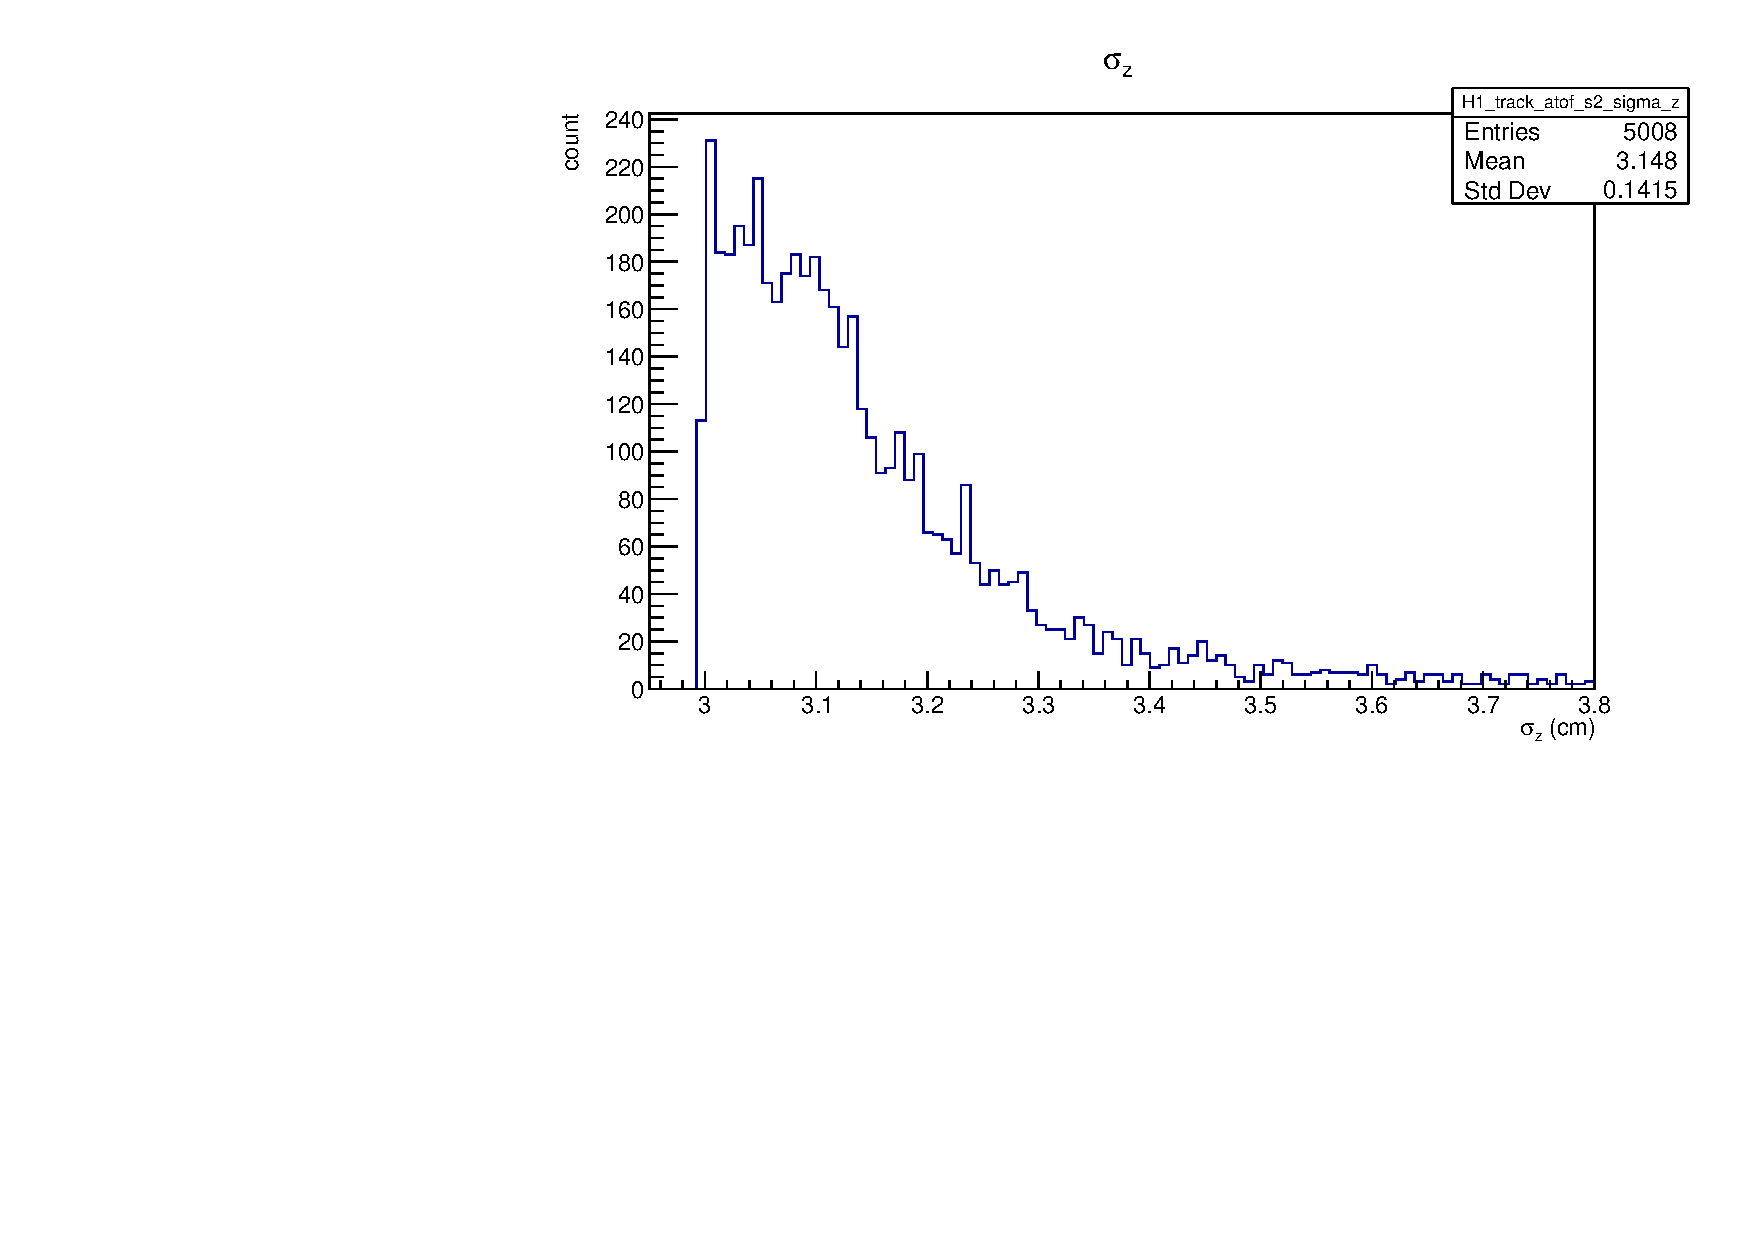
\includegraphics[width=\linewidth]{figures/sigma_z.pdf}
        \end{subfigure}
        \begin{subfigure}{0.4\textwidth}
            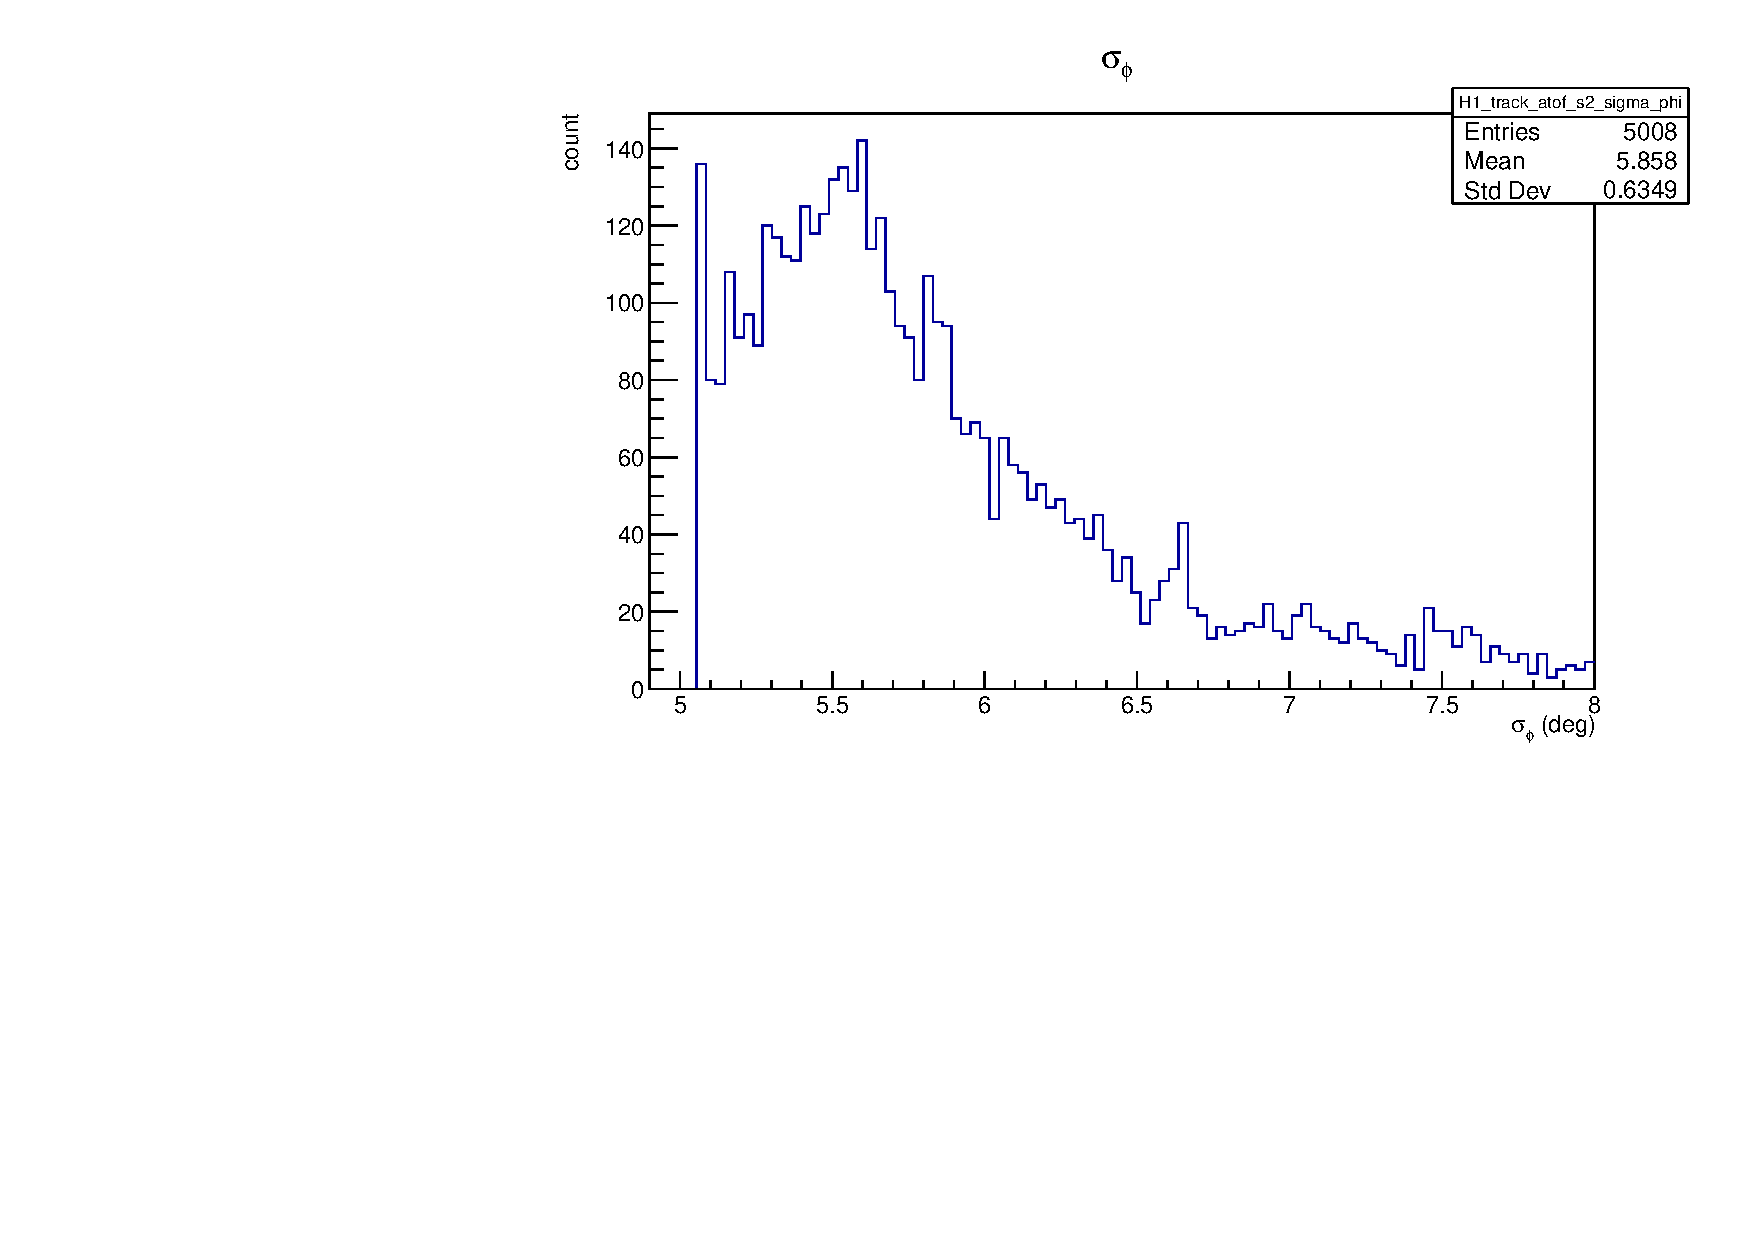
\includegraphics[width=\linewidth]{figures/sigma_phi.pdf}
        \end{subfigure}
    \end{figure}
\end{frame}




\end{document}


